\chapter{Chapter 3: Priors}
\section{Section 3.1: Introduction}
In this chapter we will consider different approaches about how to construct or choose a suitable prior distribution $\pi(\theta)$ for our parameter of interest $\theta$.  

For example, why did we use a $\mathrm{Beta}(77,5)$ distribution for $\theta$ in the music expert example (page 31)?  Why did we use a $\mathrm{Beta}(2.5,12)$ distribution for $\theta$ in the example about the video game pirate (page 34)?  And why did we assume a $\mathrm{Gamma}(10,4000)$ distribution for $\theta$ in the earthquake example (page 37)?


We will consider the case of \textit{informative priors}, where expert opinion, for example, gives us good reason to believe that some values in a permissible range for $\theta$ are more likely to occur than others.  In particular, we will revisit the examples about the music expert, the video game pirate and earthquakes in Chapter 2.  

Of course, sometimes it might be very difficult to properly elicit a prior distribution for $\theta$.  For example, there may be no expert available to help guide your choice of distribution.  In this case, the chosen prior distribution $\pi(\theta)$ might be one which keeps the mathematics simple when operating Bayes Theorem, whilst also assuming a large or ``infinite'' variance for $\theta$ (\textit{vague prior knowledge}).  Alternatively, a prior which assumes all values of $\theta$ are equally likely could be used to represent complete \textit{prior ignorance}, as in the example about the possibly biased coin (Example 2.1, page 28).   

In this chapter we will also consider the construction of priors for $\theta$ under certain parameter constraints, including the construction of \textit{truncated priors}.    




\section{Section 3.2: Informative Priors}

\paragraph{Definition 3.1: Informative Prior}{~\\
We have \emph{substantial prior information} for $\theta$ when the prior distribution {\it dominates} the posterior distribution, that is
$\pi(\theta|\underline{x})\sim\pi(\theta)$.}
\begin{figure}[h!]

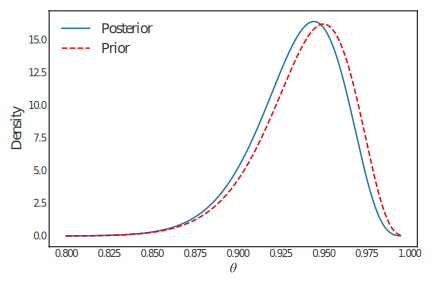
\includegraphics{images/priorposterior1.svg}
\caption{Prior (dashed) and posterior (solid) densities for the music expert's skill for the $0.8 < \theta < 1$.}
\label{fig:substantial}

\end{figure}
An example of  an informative prior was given in Example~\ref{ex:mozart} where a music expert was trying to distinguish between pages from Mozart and Haydn scores. Figure~\ref{fig:substantial} shows the prior and posterior distributions for $\theta$, the probability that the expert makes the correct choice. Notice the similarity between the prior and posterior distributions. Observing the data has not altered our beliefs about $\theta$ very much.

When we have prior information there can be some difficulties:
\begin{enumerate}
\item The practical formulation of the prior distribution from expert opinions ---
coherently specifying prior beliefs in the form of a probability
distribution is far from straightforward. This is known as \emph{prior elicitation}.
\item The intractability of the mathematics in deriving the posterior
distribution --- though with modern computing facilities this is less
of a problem,
\end{enumerate}
In the following two examples, we consider the specification of informative priors from information provided by experts. These are examples of \emph{prior elicitation}.
\clearpage

\paragraph{Example 3.1}{~\\
\label{ex:earthret}
\noindent Let us return to Example \ref{ex:earth} of Chapter 2.  Recall that we were given some data on the ``waiting times'', in days, between 21 earthquakes, and we discussed why an exponential distribution $\mathrm{Exp}(\theta)$ might be appropriate to model the waiting times.  Further, we were told that an expert on earthquakes has prior beliefs about the rate $\theta$, described by a $\mathrm{Gamma}(10,4000)$ distribution; a plot of this prior is shown in Figure \ref{fig:earthprior}.  Where did this prior distribution come from?

Suppose the expert tells us that earthquakes in the region we are interested in usually occur less than once per year; in fact, they occur on average once every 400 days.  This gives us a rate of occurrence of about 1/400 = 0.0025 per day (to match the ``daily'' units given above).  Further, he is fairly certain about this and specifies a very small variance of $6.25 \times 10^{-7}$.  

A $\mathrm{Gamma}(a,b)$ distribution seems sensible, since we can't observe a negative daily earthquake rate and the Gamma distribution is specified over positive values only.  Using the information provided by the expert, verify our use of $a=10$ and $b=4000$.}

!!dropdown!!

Recall that if $\theta \sim \mathrm{Gamma}(a,b)$, then
    \begin{align*}
        \text{E}[\theta] &= \frac{a}{b}, \\
        \text{Var}[\theta] &= \frac{a}{b^2}.
    \end{align*}
    From the prior information supplied by the expert, we must have $\text{E}[\theta] = 2.5\times 10^{-3}$ and $\text{Var}[\theta] = 6.25\times 10^{-7}$. This yields a simultaneous equation in $a$ and $b$:
    \begin{align*}
        \frac{a}{b} &= 2.5\times 10^{-3} \Rightarrow a = 2.5\times 10^{-3} b, \\
        \frac{a}{b^2} &= 6.25\times 10^{-7} \Rightarrow a = 6.25\times 10^{-7}b^2.
    \end{align*}
    Setting these two equations equal yields a quadratic equation in $b$. Since $b > 0$, we are allowed to divide both sides by $b$:
    \begin{align*}
        2.5\times 10^{-3} b &= 6.25\times 10^{-7}b^2 \\
        b &= \frac{2.5\times 10^{-3}}{ 6.25\times 10^{-7}} = 4000.
    \end{align*}
    Therefore, $a = 2.5\times 10^{-3} \times 4000 = 10$.

    So, the prior information provided by the expert is quantified correctly by $$\theta\sim\mathrm{Gamma}(10, 4000),$$ as required.

!!enddropdown!!




\paragraph{Example 3.2}{~\\
Now let us return to Example \ref{ex:mozart} of Chapter 2.  We considered an experiment to determine how good a music expert is at distinguishing between pages from Haydn and Mozart scores; when presented with a score from each composer, the expert makes the correct choice with probability $\theta$.  

Before conducting the experiment, we were told that the expert is very competent; in fact, we were told that $\theta$ should have a prior distribution peaking at around 0.95 and for which $\text{Pr}(\theta<0.8)$ is very small.  To achieve this, we assumed that $\theta \sim \mathrm{Beta}(77,5)$, with density given in Figure 2.4.  How did we know a beta distribution would be appropriate?  And how did we figure out the parameters of this distribution, i.e. $a=77$ and $b=5$?  

By now, you should understand why we might work with a beta distribution: in this example, $\theta$ is a probability and so must lie in the interval $[0,1]$, and a beta distribution is defined over this range.  But how did we know that $a=77$ and $b=5$ would give the desired properties for $\theta$?  

We are told that the mode of the distribution should be around 0.95; using the formulae on page 25, we can thus write
\begin{eqnarray}
\frac{a-1}{a+b-2}    &=& 0.95  \\
                     & &      \nonumber \\
 \Rightarrow a-1     &=&0.95(a+b-2)  \nonumber \\
 \Rightarrow a-0.95a &=&0.95b - 1.9 + 1 \nonumber \\
 \Rightarrow 0.05a   &=&0.95b - 0.9 \nonumber \\
 \Rightarrow   a     &=&19b - 18.
\end{eqnarray}
We are also told that $\text{Pr}(\theta<0.8)$ must be small.  In fact, suppose we are told that $\theta<0.8$ might occur with probability 0.0001.  This means that if we integrate the probability density function for our beta distribution between 0 and 0.8, we would get 0.0001; from Equation (2.1) on page 25, we can write this as
$$\int_{0}^{0.8} \frac{\theta^{a-1}(1-\theta)^{b-1}}{\mathrm{B}(a,b)} d\theta = 0.0001. $$
Now, setting $a = 19b-18$:
\begin{equation}
 \int_{0}^{0.8} \frac{\theta^{(19b-18)-1}(1-\theta)^{b-1}}{\mathrm{B}(19b-18,b)} d\theta = 0.0001.
\end{equation}
We have set the cumulative distribution function for a $\mathrm{Beta}(19b-18,b)$ random variable, evaluated at 0.8, equal to 0.0001 and solve for $b$.  Although this would be rather tricky to do by hand, we can do this quite easily in \texttt{R}.  Recall that the \texttt{R} command \texttt{dbeta(x,a,b)} evaluates the density of the $\mathrm{Beta}(a,b)$ distribution at the point \texttt{x} (see page 25); the command \texttt{pbeta(x,a,b)} evaluates the corresponding cumulative distribution function at \texttt{x}.  First of all, we re--write (3.3) to set it equal to zero:
\begin{equation}
\int_{0}^{0.8} \frac{\theta^{(19b-18)-1}(1-\theta)^{b-1}}{\mathrm{B}(19b-18,b)} d\theta -0.0001 = 0.
\end{equation}
We then write a function in \texttt{R} which computes the left-hand-side of Equation (3.4):
\begin{minted}{Python}
f = function(b) {
    output = pbeta(0.8, 19 * b - 18, b) - 0.0001
    return(output)
}
\end{minted}
The trick now is to use a numerical procedure to find the root of \texttt{answer} in the \texttt{R} function above, i.e. find the value \texttt{b} which equates \texttt{answer} to zero (as is required in Equation (3.4).  We can do this using the \texttt{R} function \texttt{uniroot(f, lower=, upper=)}, which uses a numerical search algorithm to find the root of the expression provided by the function \texttt{f}, having been given a \texttt{lower} bound and an \texttt{upper} bound to search within.  We know from the formulae on page 25 that $a,b>1$ when using expression (3.1) for the mode, so we can search for a root over some specified domain $>1$: for example, we might use \texttt{lower=1} and \texttt{upper=100}, giving:
\begin{minted}{Python}
uniroot(f, lower=1, upper=100)
$root
[1] 5.06513

$f.root
[1] 6.008134e-09

$iter
[1] 14

$estim.prec
[1] 6.103516e-05
\end{minted}















Thus, the solution to Equation (3.3) is $b=5.06513$.  For simplicity, rounding down to $b=5$ and then substituting into (3.2) gives
$$
a = 19 \times 5 -18 = 77,
$$
hence the use of $\theta \sim \mathrm{Beta}(77,5)$ in Example \ref{ex:mozart} in Chapter 2.}

There are many more advanced approaches of \emph{prior elicitation} and it is still an active area of research.

\clearpage



















































































 



























































































\section{Section 3.3: Parameter constraints}

Many probability models have constraints on their parameters. For example, if we are interested in the \emph{variance} $\sigma^2$ of independent normally distributed data
$$ X_i\,|\, \sigma^2 \sim \mathcal{N}(0, \sigma^2), \quad i = 1,2,\ldots,n, $$
then we must necessarily have $\sigma^2 > 0$. This is an example of a \emph{parameter constraint}. Other examples include the $a,b > 0$ parameters that are used in the $\mathrm{Gamma}(a,b)$ distribution, or the parameter $p$ used in the $\mathrm{Binomial}(n,p)$ distribution.

In order to perform \emph{Bayesian inference} on parameters which are constrained, we need to specify prior distributions which place zero probability on the regions for which the parameter can't take. 




A general approach to define priors which satisfy such constraints is by using \emph{truncated distributions}.

\paragraph{Definition 3.2: Truncated Distribution}{~\\
  Consider a univariate continuous distribution with density $\pi(\theta)$.
  Then this distribution \emph{truncated to the interval} $[a,b]$ has density:
  $$
  \pi_T(\theta) =
    \begin{cases}
      \pi(\theta) / k & \text{for } \theta \in [a,b] \\
      0 & \text{otherwise}
    \end{cases}
  $$
  where $k = \int_a^b \pi(\theta) d\theta$.}

Notes:
\begin{enumerate}
\item
For one-side constraints, for example $\theta \geq 1$, we can take $a=-\infty$ or $b=\infty$.
\item
Strict inequalities such as $\theta>1$ can be treated in exactly the same way as non-strict inequalities such as $\theta \geq 1$ (this is because $\theta$ is a continuous random variable).
\item
For Bayesian analysis we usually don't need to actually calculate $k$, as we can simply use:
$$
\pi_T(\theta) \propto
  \begin{cases}
    \pi(\theta) & \text{for } \theta \in [a,b] \\
    0 & \text{otherwise}
  \end{cases}
$$
\end{enumerate}
\clearpage
\paragraph{Example 3.3}{~\\
Suppose $\theta \sim \mathcal{N}(b,d^2)$.
Find the density of the truncated distribution for $\theta>0$.



!!dropdown!!

From the definition of a truncated distribution, we have, for $\theta >0$:
    $$ \pi_T(\theta) = \frac{1}{k \sqrt{2\pi d^2}}\exp\left[-\frac{1}{2d^2}(\theta - b)^2\right], $$
    where $k = \int_0^\infty \pi(\theta).$ Note that 
    \begin{align*}
       k = \int_0^\infty \pi(\theta) &= \text{Pr}(\theta > 0) \\
       &= 1 - \text{Pr}(\theta < 0) \\
       &= 1 - \text{Pr}\left(\frac{\theta - b}{d} < -\frac{b}{d}\right) \\
       &= 1 - \text{Pr}\left(Z < -\frac{b}{d} \right) \\
       &= 1 - \Phi\left(-\frac{b}{d}\right).
    \end{align*}
    Here, $Z \sim \mathcal{N}(0,1)$ and $\Phi(z) = \text{Pr}(Z < z)$ is the cdf of $Z$. Therefore, for $\theta > 0$:
    $$\pi_T(\theta)  = \frac{1}{\left(1 - \Phi\left(-\frac{b}{d}\right)\right) \sqrt{2\pi d^2}}\exp\left[-\frac{1}{2d^2}(\theta - b)^2\right] $$

!!enddropdown!!}

Figure~\ref{fig:normaltrunc} shows a plot of the densities of (a) a $\mathcal{N}(1,1)$
distribution and (b) a $\mathcal{N}(1,1)$ distribution truncated to $\theta>0$.
Notice that for $\theta>0$ the truncated normal's density
has the same shape as that of the original distribution.
However the truncated density takes proportionately larger values,
since both curves must have an area underneath of one.
Also, we can see that the mean of the truncated distribution will be larger than the mean of the original distribution and the standard deviation will be smaller.

This is an important general point.
Truncating a distribution changes the mean and variance.
Calculating the new values can be difficult.

\begin{figure}[ht]

\psfrag{x}{$\theta$}
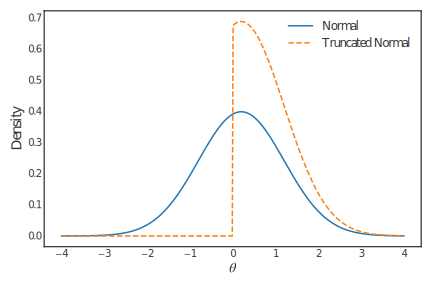
\includegraphics{images/truncatednormal.svg}
\caption{Plot of a normal and truncated normal distribution}
\label{fig:normaltrunc}

\end{figure}


\subsection*{Bayesian Inference with Truncated Priors}

Suppose we can do a Bayesian analysis for an ordinary prior.
Then it's easy to do the analysis for a truncated version of this prior by the following theorem.

\paragraph{Theorem 3.1: Truncated Posterior}{\label{theorem: truncated posterior} ~\\ 
Suppose that for a prior $\pi(\theta)$ the resulting posterior is $\pi(\theta | \underline{x})$.
Let $\pi_T(\theta)$ be the result of truncating the prior to $[a,b]$.
Then the corresponding posterior is $\pi(\theta | \underline{x})$ truncated to $[a,b]$.
\paragraph{Proof}{Theorem}{\ref{theorem: truncated posterior}}
Let $\pi'(\theta | \underline{x})$ be the posterior for the truncated prior. Then:
\begin{align*}
\pi'(\theta | \underline{x}) &\propto \pi_T(\theta) f(\underline{x}|\theta) \\
& \propto
\begin{cases}
  \pi(\theta) f(\underline{x}|\theta) & \text{for } \theta \in [a,b] \\
  0 & \text{otherwise}
\end{cases} \\
& \propto
\begin{cases}
  \pi(\theta | \underline{x}) & \text{for } \theta \in [a,b] \\
  0 & \text{otherwise}.
\end{cases}
\end{align*}

This result makes it easy to do Bayesian analysis under parameter constraints.}


















\clearpage
\paragraph{Example 3.4}{~\\
Consider again the case of $X_i|\theta\sim \mathcal{N}(\theta,h^2)$, $i=1,2,\ldots,n$
(independent) and $\theta\sim \mathcal{N}(b,d^2)$, with $h$ known.
Suppose we knew in advance that the experiment could only result in positive values for $\theta$.
Find the posterior distribution for $\theta$.

!!dropdown!!

From the previous theorem, we first compute the posterior distribution using the non-truncated prior and then we can truncate the posterior. Recall from Example 2.7 that if we use a non-truncated prior $\theta \sim\mathcal{N}(b,d^2)$, we have:
    $$ \theta | \underline{x} \sim \mathcal{N}(M, V), $$
    where
    \begin{align*}
        M &= \left(\frac{n}{h^2} + \frac{1}{d^2}\right)^{-1}\left(\frac{n\bar{x}}{h^2} + \frac{b}{d^2}\right), \\
        V &= \left(\frac{n}{h^2} + \frac{1}{d^2}\right)^{-1}.
    \end{align*}
    The posterior using the truncated prior thus has density, for $\theta > 0$:
    \begin{align*}
        \pi'(\theta | \underline{x}) = \frac{1}{\left(1 - \Phi\left(-\frac{M}{\sqrt{V}}\right)\right) \sqrt{2\pi V}}\exp\left[-\frac{1}{2V}(\theta - M)^2\right].
    \end{align*}

!!enddropdown!!

Figure~\ref{fig:posttrunc} plots the $\mathcal{N}(1,1)$ posterior densities
using the original and truncated priors.
This plot highlights an important consequence of using truncated
distributions for modelling prior beliefs, namely, that if particular
parameter values are ruled out prior to seeing the data then they are
also ruled out after seeing the data. Normally, this is not a problem
but, as the following example shows, when the truncation in a prior
distribution does not include parameter values for which the
likelihood function is large, misleading conclusions can be made.

\begin{figure}[h!]

\psfrag{x}{$\theta$}
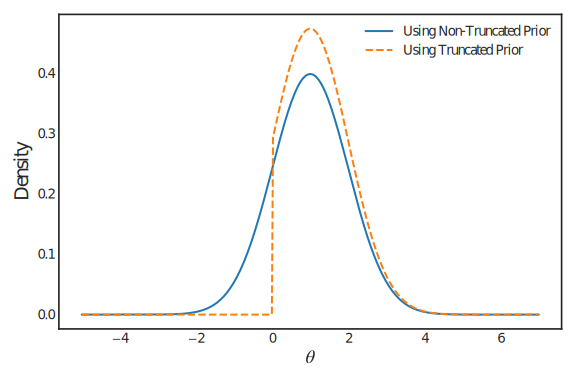
\includegraphics{images/truncposterior.svg}
\caption{Plot of a posterior distribution determined using a
non-truncated and a truncated prior distribution}
\label{fig:posttrunc}

\end{figure}}
\clearpage
\paragraph{Example 3.5}{~\\
Consider the case of a large random sample ($n=1500$) with sample mean
$\bar x=157/15\simeq 10.47$ from a normal distribution with known
variance ($h^2=100$) and a normal $\mathcal{N}(3,1)$ prior distribution for the
mean parameter~$\theta$. The prior probability that $\theta$ exceeds~9
is almost zero: $\text{Pr}(\theta>9)\simeq 10^{-9}$. So what is the effect of
using a prior distribution which rules out the extremely unlikely
values of $\theta$ greater than~9? Put another way, is there much
difference between the posterior distributions calculated using the
prior with $\text{Pr}(\theta>9)\simeq 10^{-9}$ or a truncated version of the
prior with $\text{Pr}(\theta>9)=0$?

If no truncation is applied to the prior distribution then Bayes
Theorem produces the posterior distribution $\theta|\underline{x}\sim \mathcal{N}(10,0.25^2)$. The discussion preceding this example tells us that imposing the truncation $\theta<9$ on the prior distribution produces a posterior distribution which is a $\mathcal{N}(10,0.25^2)$ distribution, truncated to $\theta<9$.  Figure~\ref{fig:posttrunc2} shows the resulting posterior densities. Clearly, truncating the prior distribution to $\theta<9$ has resulted in a posterior distribution truncated to $\theta<9$, even though the likelihood function is very peaked at $\theta\simeq 10.47$. So our prior has ruled out the most likely values according to the data! Using a prior distribution which gives very small -- but non-zero -- probability to values of $\theta>9$, avoids this problem.
\begin{figure}[h!]

\psfrag{x}{$\theta$}
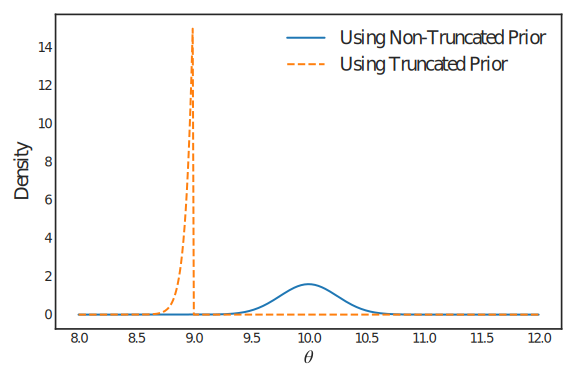
\includegraphics{images/truncposterior2.svg}
\caption{Plot of a posterior distribution determined using a
non-truncated and a truncated prior distribution}
\label{fig:posttrunc2}

\end{figure}}

This example motivates the pragmatic rule:
never rule out values for parameters which are very implausible but not impossible.
Instead these parameter values should be given very small probability density.
The data will then be allowed to inform the posterior distribution about values of $\theta$
with very low prior probability (density) but with very high likelihood.

\begin{tcolorbox}[colback=niceblue, colframe=niceblue]
\noindent \textit{``If a decision-maker thinks something cannot be true and interprets this to mean it has zero probability, he will never be influenced by any data, which is surely absurd. So leave a little probability for the moon being made of green cheese; it can be as small as 1 in a million, but have it there since otherwise an army of astronauts returning with samples of the said cheese will leave you unmoved''} \emph{-- Dennis Lindley}
\end{tcolorbox}

\clearpage
\section{Section 3.4: Uninformative Priors}
If we have very little or no prior information about the model parameters $\theta$, we must still choose a prior distribution in order to operate Bayes Theorem. Obviously, it would be sensible to choose a prior distribution which is not concentrated about any particular value, that is, one with a very large variance. In particular, most of the information about $\theta$ will be passed through to the posterior distribution via the data, and so we have $\pi(\theta|\underline{x})\sim f(\underline{x}|\theta)$.

An example of vague prior knowledge was given in Example \ref{ex:coin} where a possibly biased coin was assessed. Figure \ref{fig:little} shows the prior and posterior distributions for $\theta=\text{Pr(Head)}$. Notice that the prior and posterior distributions look very different. In fact, in this example, the posterior distribution is simply a scaled version of the likelihood function -- likelihood functions are not usually proper probability (density) functions and so scaling is required to ensure that it integrates to one. Most of our beliefs about $\theta$ have come from observing the data.

\begin{figure}[ht]

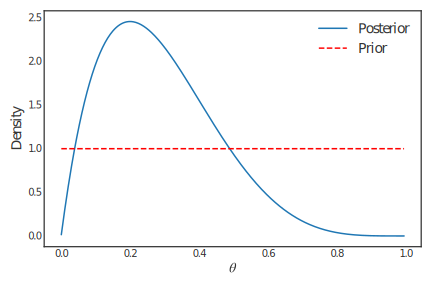
\includegraphics{images/priorplot1.svg}
\caption{Prior (dashed) and posterior (solid) densities for $\theta$}
\label{fig:little}

\end{figure}

 
\subsection*{Vague Prior Knowledge}
We represent vague prior knowledge by using a prior distribution which is conjugate to the model for $\underline{x}$ and which has ``infinite'' variance.

\paragraph{Example 3.6}{~\\
Suppose we have a random sample from a $\mathcal{N}(\mu,1/\tau)$ distribution (with $\tau$ known). Determine the posterior distribution assuming a vague prior for $\mu$.

!!dropdown!!

The conjugate prior distribution is a normal distribution. We have already seen that if the prior is $\mu\sim \mathcal{N}(b,1/d)$ then the posterior distribution is $\mu|\underline{x}\sim \mathcal{N}(B,1/D)$ where
            \begin{equation*}
                B=\frac{db+n\tau\bar x}{d+n\tau}\qquad\text{and}\qquad
                D=d+n\tau.
            \end{equation*}
        If we now make our prior knowledge vague about $\mu$ by letting the prior variance tend to infinity ($d\to 0$), we obtain
        $$
        B\to\bar x\qquad\text{and}\qquad D\to n\tau.
        $$
        Therefore, assuming vague prior knowledge for $\mu$ results in a $\mathcal{N}(\bar x,1/(n\tau))$ posterior distribution.  Notice that the posterior mean is the sample mean (the likelihood mode) and that the posterior variance $1/D\to 0$ as $n\to\infty$.

!!enddropdown!!}



\paragraph{Example 3.7}{~\\
Suppose we have a random sample from an exponential distribution, that is, $X_i|\theta\sim \mathrm{Exp}(\theta)$, $i=1,2,\ldots,n$ (independent). Determine the posterior distribution assuming a vague
prior for $\theta$.

!!dropdown!!

The conjugate prior distribution is a Gamma distribution. Recall that a $\mathrm{Gamma}(g,h)$ distribution has mean $m=g/h$ and variance $v=g/h^2$. Rearranging these formulae we obtain
        \begin{equation*}
        g=\frac{m^2}{v}\quad\quad\text{and}\quad\quad h=\frac{m}{v}. 
        \end{equation*}
        Clearly $g\to 0$ and $h\to 0$ as $v\to\infty$ (for fixed~$m$).  We have seen how taking a $\mathrm{Gamma}(g,h)$ prior distribution results in a $\mathrm{Gamma}(g+n,h+n\bar x)$ posterior distribution. Therefore, taking a vague prior distribution will give a $\mathrm{Gamma}(n,n\bar x)$ posterior distribution. 
        
        Note that the posterior mean is $1/\bar x$ (the likelihood mode) and that the posterior variance $1/(n\bar x^2)\to 0$ and $n\to\infty$.

!!enddropdown!!}

\clearpage

\subsection*{Prior Ignorance}
We could represent ignorance by the concept ``all values of $\theta$ are equally likely''. If $\theta$ were discrete with $m$ possible values then we could assign each value the same probability $1/m$. However, if $\theta$ is continuous, we need some limiting argument (from the discrete case). Suppose that $\theta$ can take values between $a$ and $b$, where $-\infty<a<b<\infty$. Letting all (permitted) values of $\theta$ be equally likely results in taking a uniform $U(a,b)$ distribution as our prior distribution for~$\theta$. However, if the parameter space is not finite then we cannot do this: there is no such thing as a $U(-\infty,\infty)$ distribution. Convention suggests that we should use the ``improper'' uniform prior distribution
\begin{equation*}
\pi(\theta)=constant.
\end{equation*}
This distribution is improper because $\int_{-\infty}^\infty \pi(\theta)\,d\theta$ is not a convergent integral, let alone equal to~one. We have a similar problem if~$\theta$  takes positive values --- we cannot use a $U(0,\infty)$ prior distribution. Now if $\theta\in (0,\infty)$ then $\phi=\log\theta\in (-\infty,\infty)$, and so we could use an ``improper'' uniform prior for $\phi$: $\pi(\phi)=constant$. In turn, this induces a distribution on $\theta$. Recall the result from Distribution Theory:

Suppose that $X$ is a random variable with probability density function $f_X(x)$. If $g$ is a bijective (1--1) function then the random variable $Y=g(X)$ has probability density function
\begin{equation}
\label{eq:p14}
f_Y(y)=f_X\left(g^{-1}(y)\right)\left|\frac{d}{dy}\,g^{-1}(y)\right|.
\end{equation}

Applying this result to $\theta=e^\phi$ gives
\begin{align*}
\pi_\theta(\theta)
&=\pi_\phi(\log\theta)\left|\frac{d}{d\theta}\,\log\theta\right|,
\quad\quad\theta>0 \\
&=constant\times\left|\frac{1}{\theta}\right|,\quad\quad\theta>0 \\
&\propto\frac{1}{\theta},\quad\quad\theta>0.
\end{align*}
This too is an improper distribution.

There is a drawback of using uniform or improper priors to represent prior ignorance: if we are ``ignorant'' about $\theta$ then we are also ``ignorant'' about any function of $\theta$, for example, about
$\phi_1=\theta^3$, $\phi_2=e^\theta$, $\phi_3=1/\theta$,
\ldots~. Is it possible to choose a distribution where we are ignorant about all these functions of~$\theta$? If not, on which function of $\theta$ should we place the uniform/improper prior distribution? After a little thought, it should be clear that there is no distribution which can represent ignorance for all functions of $\theta$. The above example shows that assigning a uniform/ignorance prior to $\theta$ means that we do not have a uniform/ignorance prior for $e^\theta$.

A solution to problems of this type was suggested by Sir~Harold Jeffreys. His suggestion was specified in terms of Fisher's Information:
\begin{equation}
\label{eq:fisher}
I(\theta)=E_{\underline{X}|\theta}\left[-
\frac{\partial^2}{\partial\theta^{2}}\,
\log f(\underline{X}|\theta)\right].
\end{equation}
He recommended that we represent prior ignorance by the prior distribution
\begin{equation}
\pi(\theta)\propto \sqrt{I(\theta)}.
\end{equation}
Such a prior distribution is known as a Jeffreys prior distribution.

\paragraph{Example 3.8}{~\\
Suppose we have a random sample from a distribution with probability \label{ex:37} density function
\begin{equation*}
f(x|\theta)=\frac{2x\,e^{-x^2/\theta}}{\theta},\quad\quad x>0,~\theta>0.
\end{equation*}
Determine the Jeffreys prior for this model.

!!dropdown!!

The likelihood function is
        \begin{align*}
        f(\underline{x}|\theta) 
        &=\prod_{i=1}^n \frac{2x_i\,e^{-x_i^2/\theta}}{\theta} \\
        &=\frac{2^n}{\theta^n}\left(\prod_{i=1}^n x_i\right)
        \exp\left\{-\frac{1}{\theta}\sum_{i=1}^n x_i^2\right\}.
        \end{align*}
        Therefore, the log-likelihood function is
        \begin{align*}
            \log f(\underline{x} | \theta) &= n\log 2 - n\log \theta + \sum_{i=1}^n\log(x_i) - \frac{1}{\theta}\sum_{i=1}^n x_i^2.
        \end{align*}
        The derivatives are:
        \begin{align*}
            \frac{\partial}{\partial \theta}\log f(\underline{x} | \theta) &= -\frac{n}{\theta} + \frac{1}{\theta^2}\sum_{i=1}^n x_i^2, \\
            \frac{\partial^2}{\partial \theta^2}\log f(\underline{x} | \theta) &= \frac{n}{\theta^2} - \frac{2}{\theta^3}\sum_{i=1}^n x_i^2.
        \end{align*}
        The Fisher information is then
        \begin{align*}
            I(\theta) &= -\text{E}_{\underline{X}|\theta}\left[ \frac{n}{\theta^2} - \frac{2}{\theta^3} \sum_{i=1}^n X_i^2  \right] \\
            &= -\frac{n}{\theta^2} + \frac{2}{\theta^3}\sum_{i=1}^n \text{E}[X_i^2|\theta].
        \end{align*}

!!enddropdown!!

\clearpage

!!dropdown!!

\begin{align*}
        E\left[X^2 \,| \, \theta\right]
        &=\int_0^\infty x^2\times
        \left(\frac{2x\,e^{-x^2/\theta}}{\theta}\right)\, \mathrm{d}x \\
        &=\theta\int_0^\infty y\,e^{-y}\,\mathrm{d}y 
        \quad\quad\text{using the substitution } y=x^2/\theta \\
        &=\theta\times 1 \\
        &=\theta.
        \end{align*}
        Therefore
        $$
        I(\theta)
        =-\frac{n}{\theta^2}+\left(\frac{2n}{\theta^3}\times\theta\right) 
        =\frac{n}{\theta^2}.
        $$
        Hence, the Jeffreys prior for this model is
        \begin{align*}
        \pi(\theta)&\propto I(\theta)^{1/2} \\
        &\propto \frac{\sqrt{n}}{\theta},\quad\quad\theta>0 \\
        &\propto \frac{1}{\theta},\quad\quad\theta>0.
        \end{align*}

!!enddropdown!!


Notice that this distribution is improper since $\int_0^\infty d\theta/\theta$ is a divergent integral, and so we cannot find a constant which ensures that the density function integrates to one.}

\clearpage

\paragraph{Example 3.9}{~\\
Suppose we have a random sample from an exponential distribution, that \label{ex:38} is, $X_i|\theta\sim \mathrm{Exp}(\theta)$, $i=1,2,\ldots,n$ (independent). Determine the Jeffreys prior for this model.

!!dropdown!!

Recall that the likelihood function is
    $f_{\underline{X}}(\underline{x}|\theta)=\theta^n e^{-n\bar x\theta}$,
    and therefore 
    \begin{align*}
    \log f_{\underline{X}}(\underline{x}|\theta) &=n\log\theta -n\bar x\theta \\
    \frac{\partial}{\partial\theta} \log
    f_{\underline{X}}(\underline{x}|\theta) &=\frac{n}{\theta}-n\bar x \\
    \frac{\partial^2}{\partial\theta^2} \log
    f_{\underline{X}}(\underline{x}|\theta)&=-\frac{n}{\theta^2} \\ 
    \Rightarrow I(\theta) &=E_{\underline{X}|\theta}
    \left[-\frac{\partial^2}{\partial\theta^2} \log
    f_{\underline{X}}(\underline{x}|\theta)\right]=\frac{n}{\theta^2}.
    \end{align*}
    Hence, the Jeffreys prior for this model is
    \begin{align*}
    \pi(\theta)&\propto I(\theta)^{1/2} \\
    &\propto \frac{\sqrt{n}}{\theta},\quad\quad\theta>0 \\
    &\propto \frac{1}{\theta},\quad\quad\theta>0.
    \end{align*}

!!enddropdown!!

Notice that this distribution is improper since $\int_0^\infty d\theta/\theta$ is a divergent integral, and so we cannot find a constant which ensures that the density function integrates to one.

Notice also that this density is, in fact, a limiting form of a $\mathrm{Gamma}(g,h)$ density (ignoring the integration constant) since
\begin{equation*}
\frac{h^g\,\theta^{g-1}e^{-h\theta}}{\Gamma(g)}\propto
\theta^{g-1}e^{-h\theta} 
\to \frac{1}{\theta},\quad\quad\text{as }g\to 0,~h\to 0.
\end{equation*}
Therefore, we obtain the same posterior distribution whether we adopt the Jeffreys prior or vague prior knowledge.}

\clearpage

\paragraph{Example 3.10}{~\\
Suppose we have a random sample from a $\mathcal{N}(\mu,1/\tau)$ distribution \label{ex:39} (with $\tau$ known). Determine the Jeffreys prior for this model.

!!dropdown!!

Recall that the likelihood function is
    $$
    f_{\underline{X}}(\underline{x}|\mu)=
    \left(\frac{\tau}{2\pi}\right)^{n/2}
    \exp\left\{-\frac{\tau}{2}\sum_{i=1}^n (x_i-\mu)^2\right\},
    $$
    and therefore 
    \begin{align*}
    \log\,&f_{\underline{X}}(\underline{x}|\mu)=\frac{n}{2}\log(\tau)-\frac{n}{2}\log(2\pi)
    -\frac{\tau}{2}\sum_{i=1}^n (x_i-\mu)^2 \\
    &\Rightarrow\quad \frac{\partial}{\partial\mu} \log
    f_{\underline{X}}(\underline{x}|\mu)=-\frac{\tau}{2}\times\sum_{i=1}^n -2(x_i-\mu)\\
    &\phantom{\Rightarrow\quad \frac{\partial}{\partial\mu} \log f_{\underline{X}}(\underline{x}|\mu)}
    =\tau\sum_{i=1}^n (x_i-\mu) \\
    &\phantom{\Rightarrow\quad \frac{\partial}{\partial\mu} \log f_{\underline{X}}(\underline{x}|\mu)}
    =n\tau(\bar x-\mu)\\
    &\Rightarrow\quad \frac{\partial^2}{\partial\mu^2} \log
    f_{\underline{X}}(\underline{x}|\mu)=-n\tau\\
    &\Rightarrow\quad I(\mu)=E_{\underline{X}|\mu}
    \left[-\frac{\partial^2}{\partial\mu^2} \log
    f_{\underline{X}}(\underline{x}|\mu)\right]=n\tau.
    \end{align*}
    Hence, the Jeffreys prior for this model is
    \begin{align*}
    \pi(\mu)&\propto I(\mu)^{1/2} \\
    &\propto\sqrt{n\tau},\qquad-\infty<\mu<\infty \\
    &= constant,\qquad-\infty<\mu<\infty. 
    \end{align*}

!!enddropdown!!

Notice that this distribution is improper since $\int_{-\infty}^\infty d\mu$ is a divergent integral, and so we cannot find a constant which ensures that the density function integrates to one.

Also it is a limiting form of a $\mathcal{N}(b,1/d)$ density (ignoring the integration constant) since
\begin{equation*}
\left(\frac{d}{2\pi}\right)^{1/2}\exp\left\{-\frac{d}{2}(\mu-b)^2\right\}
\propto
\exp\left\{-\frac{d}{2}(\mu-b)^2\right\}
\to 1,\quad\quad\text{as }d\to 0.
\end{equation*}
Therefore, we obtain the same posterior distribution whether we adopt
the Jeffreys prior or vague prior knowledge.}

\clearpage

As discussed at the beginning of this section on prior ignorance, Jeffrey's prior is \textbf{\color{darkblue}invariant to reparameterisation}. The following example demonstrates an instance of this:

\paragraph{Example 3.11}{Recall that, from Example 3.9, the Jeffreys prior for the model
    $$ X_i|\theta\sim \mathrm{Exp}(\theta), \quad i = 1,\ldots, n $$
    is
    $$ \pi(\theta) \propto \frac{1}{\theta}. $$
    Suppose we instead \textbf{\color{darkblue}reparameterised} our model and instead used the parameter $\phi = \log \theta$. First, using Jeffrey's prior for $\theta$ compute the density of the transformed random variable $\phi = \log\theta$. 
    
    Finally, compute Jeffrey's prior using $\phi$ as the parameter, where each $X_i|\phi \sim \mathrm{Exp}(e^{\phi})$.
    
    !!dropdown!!

Recall the change of variable formula:  If $\theta$ is a random variable and $\phi = g(\theta)$ for a bijective and differentiable function $g$, then
        $$ \pi_{\phi}(\phi) = \pi_{\theta}(g^{-1}(\phi))\left|\frac{\partial}{\partial \phi} g^{-1}(\phi)\right|. $$
        We have $g(\theta) = \log\theta$ and so $g^{-1}(\phi) = e^{\phi}$ and $\frac{\partial}{\partial\phi}  \left(e^{\phi}\right) = e^{\phi}.$
        Therefore, the density of $\phi = \log \theta$ is
        $$ \pi_{\phi}(\phi) \propto \frac{1}{e^{\phi}} \times e^{\phi}  = 1.$$

        The likelihood function of the model $X_i|\phi \sim \mathrm{Exp}(e^{\phi}), \quad i=1,\ldots,n$ is
         \begin{align*}
             f(\underline{x}|\phi) &= \prod_{i=1}^n e^{\phi} e^{-e^{\phi}x_i} = e^{n\phi} \exp\left\{-n\bar{x}e^{\phi}\right\}.
         \end{align*}
         We have $\log f(\underline{x}|\phi) = n\phi -  n\bar{x}e^{\phi}.$
         The second derivative with respect to $\phi$ is
         $$ \frac{\partial^2}{\partial\phi^2} \log f(\underline{x}|\phi) = - n\bar{x}e^{\phi}.$$
         Therefore, Fishers information is
        \begin{align*}
            I(\phi) &= -\text{E}_{\underline{X}|\phi}\left[\frac{\partial^2}{\partial\phi^2} \log f(\underline{x}|\phi) \right] \\
            &= \text{E}_{\underline{X}|\phi}[n\bar{X}e^{\phi}].
        \end{align*}
        Note that $$\text{E}[X_i] = e^{-\phi}$$ and so $I(\phi) = n e^{-\phi} e^{\phi} = n$. Therefore, Jeffreys prior is
        $\pi(\phi) \propto \sqrt{I(\phi)} = 1$.

!!enddropdown!!}

\clearpage


\section{Section 3.5: Asymptotic posterior distribution}
There are many limiting results in Statistics. The one you will probably remember is the Central Limit Theorem. This concerns the distribution of $\bar X_n$, the mean of $n$ independent and identically distributed random variables (each with known mean $\mu$ and known variance $\sigma^2$), as the sample size $n\to\infty$. It is easy to show that $\text{E}[\bar X_n]=\mu$ and $\text{Var}[\bar X_n]=\sigma^2/n$, and so 
$$
\text{E}\left[\frac{\sqrt{n}(\bar{X}_{n}-\mu)}{\sigma}\right] = 0 \qquad \mathrm{and} \qquad \text{Var}\left[\frac{\sqrt{n}(\bar{X}_{n}-\mu)}{\sigma}\right]=1.
$$
These two equations are true for all values of $n$.  The important part of the Central Limit Theorem is the description of the distribution of $\sqrt{n}(\bar{X}_{n}-\mu)/\sigma$ as $n \to \infty$: 
\begin{equation*}
\frac{\sqrt{n}(\bar X_n-\mu)}{\sigma}\stackrel{\cal D} \longrightarrow
\mathcal{N}(0,1)\quad\quad\text{as }n\to\infty.
\end{equation*}
The following theorem gives a similar result for the posterior
distribution. 

\paragraph{Theorem 3.2: Asymptotic posterior}{\label{theorem: asymptotic posterior} ~\\ 
Suppose we have a statistical model $f(\underline{x}|\theta)$ for data
$\underline{x} = (x_1, \ldots, x_n)^\top$, together with a prior distribution $\pi(\theta)$ for
$\theta$. Then
$$\sqrt{J(\hat{\theta})}~(\theta-\hat{\theta})|\underline{x} \stackrel{\cal D}
  \longrightarrow \mathcal{N}(0,1)
  \quad\quad\text{as }n\to\infty $$
    where $\hat{\theta}$ is the likelihood mode and $J(\theta)$
    is the \emph{observed information}:
    $$ J(\theta)=-\frac{\partial^2}{\partial\theta^2}\, \log f(\underline{x}|\theta).$$}
\clearpage
\paragraph{Proof}{Theorem}{\ref{theorem: asymptotic posterior}}
Using Bayes Theorem, the posterior distribution for $\theta$ is
$$\pi(\theta|\underline{x}) \propto\pi(\theta)\,f(\underline{x}|\theta).$$
Let $\psi=\sqrt{n}(\theta-\hat\theta)$ and
$$\ell_n(\theta) =\frac{1}{n}\,\log f(\underline{x}|\theta) $$
be the average log-likelihood per observation, in which
case, $f(\underline{x}|\theta)=e^{n\ell_n(\theta)}$. Using \eqref{eq:p14},
the posterior distribution of $\psi$ is
\begin{align*}
\pi_\psi(\psi|\underline{x})
&=\pi_\theta\left(\hat\theta+\left.\frac{\psi}{\sqrt{n}}\right|\underline{x}\right)
\times\frac{1}{\sqrt{n}} \\
&\propto\pi_\theta\left(\hat\theta+\frac{\psi}{\sqrt{n}}\right)
\exp\left\{n\ell_n\left(\hat\theta+\frac{\psi}{\sqrt{n}}\right)\right\}.
\end{align*}
Now taking Taylor series expansions about $\psi=0$ gives
\begin{align*}
\pi_\theta\left(\hat\theta+\frac{\psi}{\sqrt{n}}\right)
&=\pi_\theta(\hat\theta)+
\pi_\theta'(\hat\theta)\frac{\psi}{\sqrt{n}}
+O\left(\frac{\psi^2}{n}\right) \\
&=\pi_\theta(\hat\theta)\left\{1+O\left(\frac{\psi}{\sqrt{n}}\right)\right\}
\\ \\
n\ell_n\left(\hat\theta+\frac{\psi}{\sqrt{n}}\right)
&=n\left\{\ell_n(\hat\theta)+
\ell_n'(\hat\theta)\frac{\psi}{\sqrt{n}}+
\frac{1}{2}\ell_n''(\hat\theta)\frac{\psi^2}{n}
+O\left(\frac{\psi^3}{n^{3/2}}\right)\right\} \\
&=n\ell_n(\hat\theta)+\frac{1}{2}
\ell_n''(\hat\theta)\psi^2+O\left(\frac{\psi^3}{\sqrt{n}}\right) \\
\end{align*}
since $\ell_n'(\hat\theta)=0$ by definition of the maximum likelihood
estimate. Therefore, retaining only terms in $\psi$, we have
\begin{align*}
\pi_\psi(\psi|\underline{x})
&\propto
\pi_\theta(\hat\theta)\left\{1+O\left(\frac{\psi}{\sqrt{n}}\right)\right\}
\exp\left\{n\ell_n(\hat\theta)+\frac{1}{2}
\ell_n''(\hat\theta)\psi^2+O\left(\frac{\psi^3}{\sqrt{n}}\right)\right\} \\
&\propto
\exp\{n\ell_n(\hat\theta)\}
\exp\left\{\frac{1}{2}\ell_n''(\hat\theta)\psi^2\right\}
\exp\left\{O\left(\frac{\psi^3}{\sqrt{n}}\right)\right\}
\left\{1+O\left(\frac{\psi}{\sqrt{n}}\right)\right\} \\
&\propto
\exp\left\{\frac{1}{2}\ell_n''(\hat\theta)\psi^2\right\}
\left\{1+O\left(\frac{\psi^3}{\sqrt{n}}\right)\right\}
\left\{1+O\left(\frac{\psi}{\sqrt{n}}\right)\right\} \\
&\propto
\exp\left\{\frac{1}{2}\ell_n''(\hat\theta)\psi^2\right\}
\left\{1+O\left(\frac{\psi}{\sqrt{n}}\right)\right\} \\
&\propto
\exp\left\{-\frac{\psi^2}{2[-\ell_n''(\hat\theta)]^{-1}}\right\}
\left\{1+O\left(\frac{\psi}{\sqrt{n}}\right)\right\}. 
\end{align*}
Hence
$$
\pi_\psi(\psi|\underline{x})\to 
k\exp\left\{-\frac{\psi^2}{2[-\ell_n''(\hat\theta)]^{-1}}\right\}
\quad\quad\text{as }n\to\infty.
$$
Thus, the limiting form of the posterior density for $\psi$
is that of a $\mathcal{N}\left(0,[-\ell_n''(\hat\theta)]^{-1}\right)$
distribution. Hence
$$
\sqrt{n}(\theta-\hat\theta)|\underline{x}\stackrel{\cal D} \longrightarrow
\mathcal{N}\left(0,[-\ell_n''(\hat\theta)]^{-1}\right)
\quad\quad\text{as }n\to\infty,
$$
or, equivalently, since $n\ell_n(\theta)=\log f(\underline{x}|\theta)$
$$
\sqrt{J(\hat{\theta})}~\left.\bigl(\theta-\hat\theta\bigr)
\right|\underline{x}\stackrel{\cal D} \longrightarrow \mathcal{N}(0,1)
\quad\quad\text{as }n\to\infty,
$$
as required.
\subsection*{Comments}

\begin{enumerate}
\item This asymptotic result can give us a useful approximation to the
posterior distribution for $\theta$ when $n$ is large:
$$
\theta|\underline{x}\sim \mathcal{N}\left(\hat\theta,J(\hat{\theta})^{-1}
\right)
\quad\quad\text{approximately}.
$$
\item The observed information is similar to Fisher's information $\eqref{eq:fisher}$. In fact, Fisher's information is the expected value of the observed information, where the expectation is taken over the distribution of $\underline{X}|\theta$, that is, $I(\theta)=E_{\underline{X}|\theta}[J(\theta)]$.
\item This limiting result is similar to one for the maximum likelihood estimator in Frequentist Statistics:
\begin{equation}
\label{eq:mle}
\sqrt{I(\theta)}~(\hat{\theta}-\theta)|\underline{x}
\stackrel{\cal D} \longrightarrow \mathcal{N}(0,1).
\quad\quad\text{as }n\to\infty, 
\end{equation}
Note that $\eqref{eq:mle}$ is a statement about the distribution of $\hat{\theta}$ for fixed (unknown) $\theta$, whereas the Theorem is a statement about the distribution of $\theta$ for fixed (known)~$\hat{\theta}$.
\end{enumerate}

\clearpage
\paragraph{Example 3.12}{~\\
Suppose we have a random sample from a distribution with probability density function
\begin{equation*}
f(x|\theta)=\frac{2x\,e^{-x^2/\theta}}{\theta},\quad\quad x>0,~\theta>0.
\end{equation*}
Determine the asymptotic posterior distribution for~$\theta$. Note that from Example~\ref{ex:37} we have 
\begin{align*}
\frac{\partial}{\partial\theta} \log
f(\underline{x}|\theta)&=-\frac{n}{\theta}+\frac{1}{\theta^2}\sum_{i=1}^n
x_i^2, \\
J(\theta)=-\frac{\partial^2}{\partial\theta^2} \log
f(\underline{x}|\theta)&=-\frac{n}{\theta^2} +\frac{2}{\theta^3}\sum_{i=1}^n
x_i^2 =\frac{n}{\theta^3}\left(-\theta+\frac{2}{n}\sum_{i=1}^n
x_i^2\right).
\end{align*}

!!dropdown!!

Write $\overline{x^2}=\dfrac{1}{n}\displaystyle\sum_{i=1}^n x_i^2$ then we have
    \begin{align*}
    \frac{\partial}{\partial\theta} \log f(\underline{x}|\theta)=0
    \quad\quad&\Longrightarrow\quad\quad
    \hat\theta=\overline{x^2}, \\
    &\Longrightarrow\quad\quad
    J(\hat\theta)=\frac{n}{\left(\overline{x^2}\right)^2} \\
    &\Longrightarrow\quad\quad
    J(\hat\theta)^{-1}=\frac{1}{n}\left(\overline{x^2}\right)^2.
    \end{align*}
    Therefore, for large $n$, the (approximate) posterior distribution for
    $\theta$ is
    $$
    \theta|\underline{x}\sim \mathcal{N}\left(\overline{x^2},\,
    \frac{1}{n}\left(\overline{x^2}\right)^2\right).
    $$

!!enddropdown!!}



\paragraph{Example 3.13}{~\\
Suppose we have a random sample from an exponential distribution, that is, $X_i|\theta\sim \mathrm{Exp}(\theta)$, $i=1,2,\ldots,n$ (independent). Determine the asymptotic posterior distribution for $\theta$. Note that from Example \ref{ex:38} we have
\begin{align*}
\frac{\partial}{\partial\theta} \log
f(\underline{x}|\theta)&=\frac{n}{\theta}-n\bar x , \\
J(\theta)=-\frac{\partial^2}{\partial\theta^2} \log
f(\underline{x}|\theta)&=\frac{n}{\theta^2}.
\end{align*}

!!dropdown!!

We have
    \begin{align*}
    \frac{\partial}{\partial\theta} \log f(\underline{x}|\theta)=0
    \quad\quad&\Longrightarrow\quad\quad
    \hat\theta=\frac{1}{\bar x} \\
    &\Longrightarrow\quad\quad
    J(\hat\theta)=n\bar x^2 \\
    &\Longrightarrow\quad\quad
    J(\hat\theta)^{-1}=\frac{1}{n\bar x^2}.
    \end{align*}
    Therefore, for large $n$, the (approximate) posterior distribution for $\theta$ is
    $$
    \theta|\underline{x}\sim \mathcal{N}\left(\frac{1}{\bar x},\,\frac{1}{n\bar x^2}\right).
    $$

!!enddropdown!!

Recall that, assuming a vague prior distribution, the posterior
distribution is a $\mathrm{Gamma}(n,n\bar x)$ distribution, with mean $1/\bar x$
and variance $1/(n\bar x^2)$. The Central Limit Theorem tells us that,
for large $n$, the gamma distribution tends to a normal distribution,
matched, of course, for mean and variance. Therefore, we have shown
that, for large $n$, the asymptotic posterior distribution is the same
as the posterior distribution under vague prior knowledge. Not a
surprising result!}



\paragraph{Example 3.14}{~\\
Suppose we have a random sample from a $\mathcal{N}(\mu,1/\tau)$ distribution
(with $\tau$ known). Determine the asymptotic posterior distribution
for~$\mu$. Note that from Example~\ref{ex:39} we have
\begin{align*}
\frac{\partial}{\partial\mu} \log
f(\underline{x}|\mu)&=n\tau(\bar x-\mu), \\
J(\mu)=-\frac{\partial^2}{\partial\mu^2} \log
f(\underline{x}|\mu)&=n\tau.
\end{align*}



!!dropdown!!

We have
    \begin{align*}
    \frac{\partial}{\partial\mu} \log f(\underline{x}|\mu)=0
    \quad\quad&\Longrightarrow\quad\quad
    \hat\mu=\bar x \\
    &\Longrightarrow\quad\quad
    J(\hat\mu)=n\tau \\
    &\Longrightarrow\quad\quad
    J(\hat\mu)^{-1}=\frac{1}{n\tau}.
    \end{align*}
    Therefore, for large $n$, the (approximate) posterior distribution for $\mu$ is
    $$
    \mu|\underline{x}\sim \mathcal{N}\left(\bar x,\,\frac{1}{n\tau}\right).
    $$

!!enddropdown!!

Again, we have shown that the asymptotic posterior distribution is the
same as the posterior distribution under vague prior knowledge.}

